\documentclass[tikz,border=12pt]{standalone}
\usepackage{amsmath,bm}
\usetikzlibrary{positioning,arrows.meta,backgrounds,decorations.pathreplacing,calc}

\begin{document}
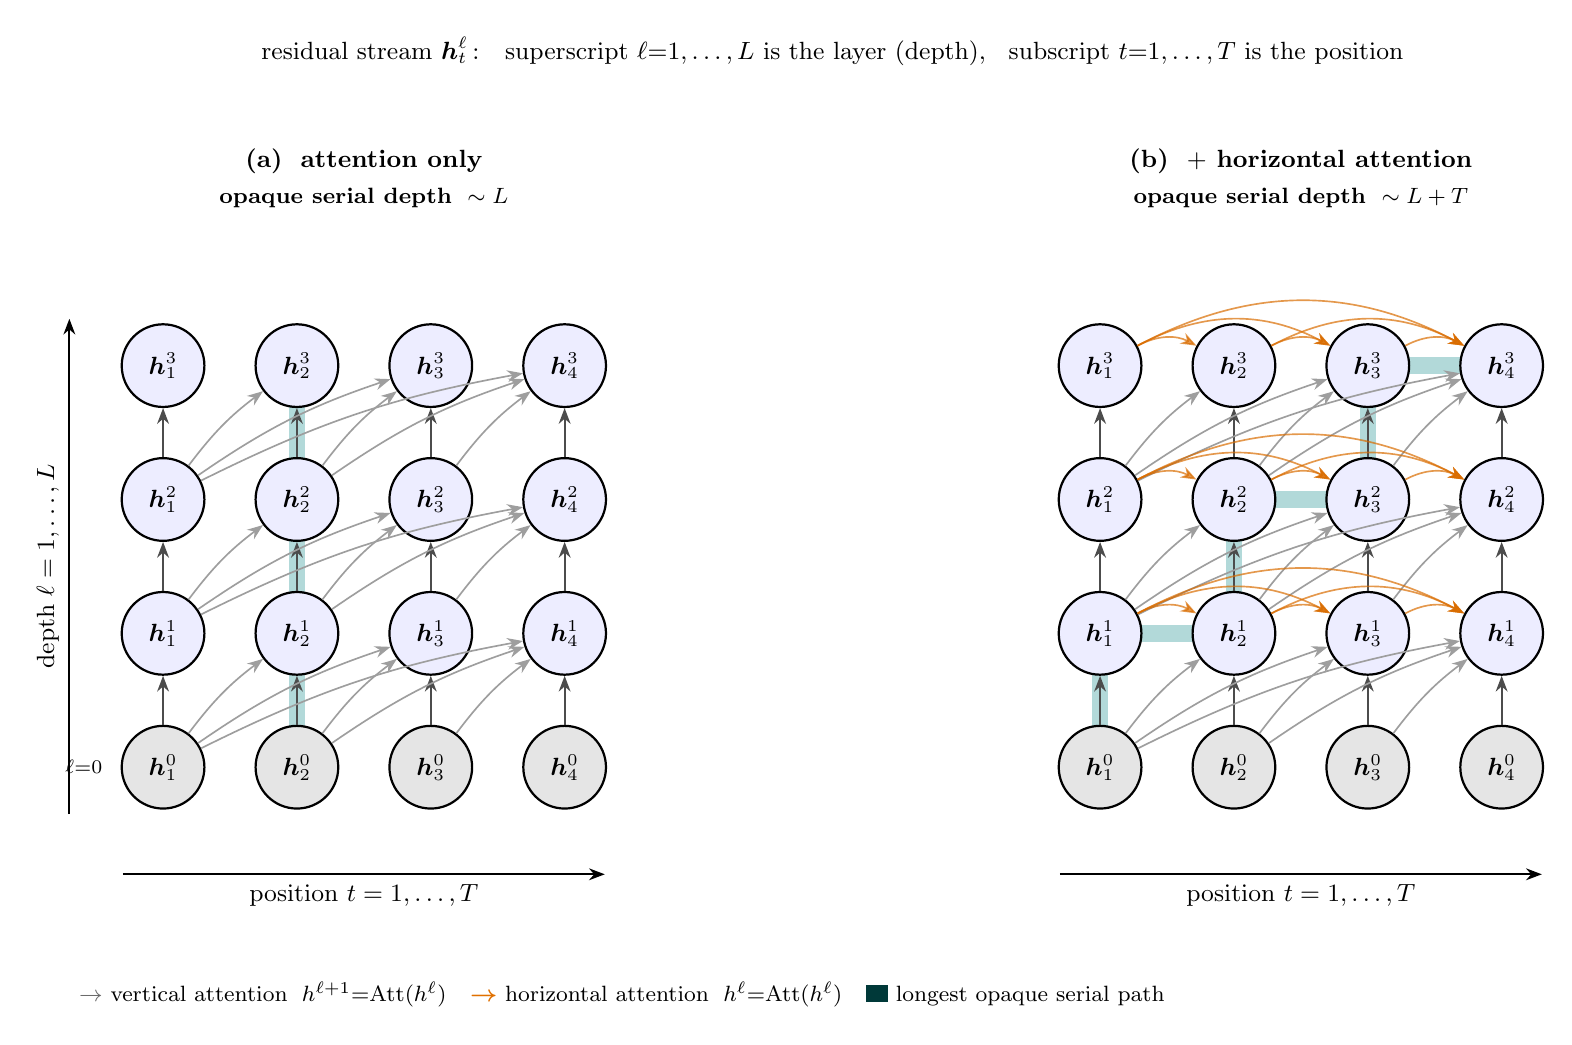
\begin{tikzpicture}[
  >={Stealth[length=2mm]},
  x=1.7cm, y=1.7cm,
  hnode/.style={circle, draw=black, thick, minimum size=10.5mm, inner sep=0pt, fill=blue!7, font=\small},
  inode/.style={circle, draw=black, thick, minimum size=10.5mm, inner sep=0pt, fill=black!10, font=\small},
  vedge/.style={->, draw=black!70, thick},                 % vertical attention: same position
  vatt/.style ={->, draw=black!38, semithick},             % vertical attention: earlier positions
  hatt/.style ={->, draw=orange!85!black, semithick, opacity=0.7},  % horizontal attention (causal fan)
  crit/.style ={line width=6pt, draw=teal!30, line cap=round, line join=round},
  ptitle/.style={font=\bfseries\small},
]
\def\T{4}\def\L{3}
\def\S{7}     % panel-b x-offset

% ============================== PANEL (a) ==============================
\foreach \l in {0,...,\L}{ \foreach \t in {1,...,\T}{
  \ifnum\l=0 \node[inode](a\l\t) at (\t,\l){$\bm h^{0}_{\t}$};
  \else      \node[hnode](a\l\t) at (\t,\l){$\bm h^{\l}_{\t}$};\fi
}}
\foreach \l in {1,...,\L}{ \pgfmathtruncatemacro{\lp}{\l-1}
  \foreach \t in {1,...,\T}{
    \draw[vedge] (a\lp\t) -- (a\l\t);
    \ifnum\t>1 \pgfmathtruncatemacro{\tm}{\t-1}
      \foreach \tp in {1,...,\tm}{ \draw[vatt] (a\lp\tp) to[bend left=8] (a\l\t); }
    \fi
}}

% ============================== PANEL (b) ==============================
\begin{scope}[shift={(\S,0)}]
  \foreach \l in {0,...,\L}{ \foreach \t in {1,...,\T}{
    \ifnum\l=0 \node[inode](b\l\t) at (\t,\l){$\bm h^{0}_{\t}$};
    \else      \node[hnode](b\l\t) at (\t,\l){$\bm h^{\l}_{\t}$};\fi
  }}
  \foreach \l in {1,...,\L}{ \pgfmathtruncatemacro{\lp}{\l-1}
    \foreach \t in {1,...,\T}{
      \draw[vedge] (b\lp\t) -- (b\l\t);
      \ifnum\t>1 \pgfmathtruncatemacro{\tm}{\t-1}
        \foreach \tp in {1,...,\tm}{ \draw[vatt] (b\lp\tp) to[bend left=8] (b\l\t); }
      \fi
  }}
  % horizontal attention: every earlier position in a layer flows into each later one
  \foreach \l in {1,...,\L}{
    \foreach \t in {2,...,\T}{ \pgfmathtruncatemacro{\tm}{\t-1}
      \foreach \tp in {1,...,\tm}{ \draw[hatt] (b\l\tp) to[bend left=28] (b\l\t); }
    }
  }
\end{scope}

% ============================== critical paths (background) ==============================
\begin{scope}[on background layer]
  \draw[crit] (a02.center) -- (a12.center) -- (a22.center) -- (a32.center);
  \draw[crit] (b01.center) -- (b11.center) -- (b12.center) -- (b22.center)
              -- (b23.center) -- (b33.center) -- (b34.center);
\end{scope}

% ============================== titles & depth annotations ==============================
\node[ptitle,align=center] at (2.5,4.4)
   {(a)\; attention only\\[2pt]\footnotesize opaque serial depth $\;\sim L$};
\node[ptitle,align=center] at (\S+2.5,4.4)
   {(b)\; $+$ horizontal attention\\[2pt]\footnotesize opaque serial depth $\;\sim L+T$};

% overall caption: index convention
\node[align=center,font=\small] at (\S/2+2.5,5.35)
   {residual stream $\bm h^{\ell}_{t}$\,:\;\; superscript $\ell{=}1,\dots,L$ is the layer (depth),\;\;
    subscript $t{=}1,\dots,T$ is the position};

% ============================== axes ==============================
% depth axis (left of panel a)
\draw[->,thick] (0.3,-0.35) -- (0.3,3.35)
   node[midway,rotate=90,anchor=south,font=\small] {depth $\ell = 1,\dots,L$};
\node[font=\scriptsize,anchor=east] at (0.62,0) {$\ell{=}0$};
% position axes (below each panel)
\foreach \ox in {0,\S}{
  \draw[->,thick] (\ox+0.7,-0.8) -- (\ox+\T+0.3,-0.8)
     node[midway,below,font=\small] {position $t = 1,\dots,T$};
}

% ============================== legend ==============================
\node[anchor=west,align=left,font=\footnotesize] at (0.3,-1.7)
 {\textcolor{black!60}{$\rightarrow$}~vertical attention $\;h^{\ell+1}{=}\mathrm{Att}(h^{\ell})$\quad
  \textcolor{orange!88!black}{$\boldsymbol\rightarrow$}~horizontal attention $\;h^{\ell}{=}\mathrm{Att}(h^{\ell})$\quad
  \textcolor{teal!45!black}{\rule{8pt}{6pt}}~longest opaque serial path};
\end{tikzpicture}
\end{document}
